\subsection{Эффект Доплера. Красное смещение}
\term{Эффект Доплера}~--- эффект изменения частоты и длины волны электромагнитного излучения, регистрируемого приёмником, вызванный относительным движением источника и приёмника (см.~Рис.\,\ref{doppler-ef}).

При $\Delta \lambda \ll \lambda_0$ с большой точностью выполняется следующее важное соотношение:\begin{equation}
\beta \equiv \dfrac{v}{c} = \dfrac{\lambda - \lambda_0}{\lambda_0} \equiv \dfrac{\Delta \lambda}{\lambda_0},
\label{eq:dopler-ef-simple}
\end{equation}
\begin{wrapfigure}[6]{r}{0.5\tw}
\centering
\vspace{-.5pc}
%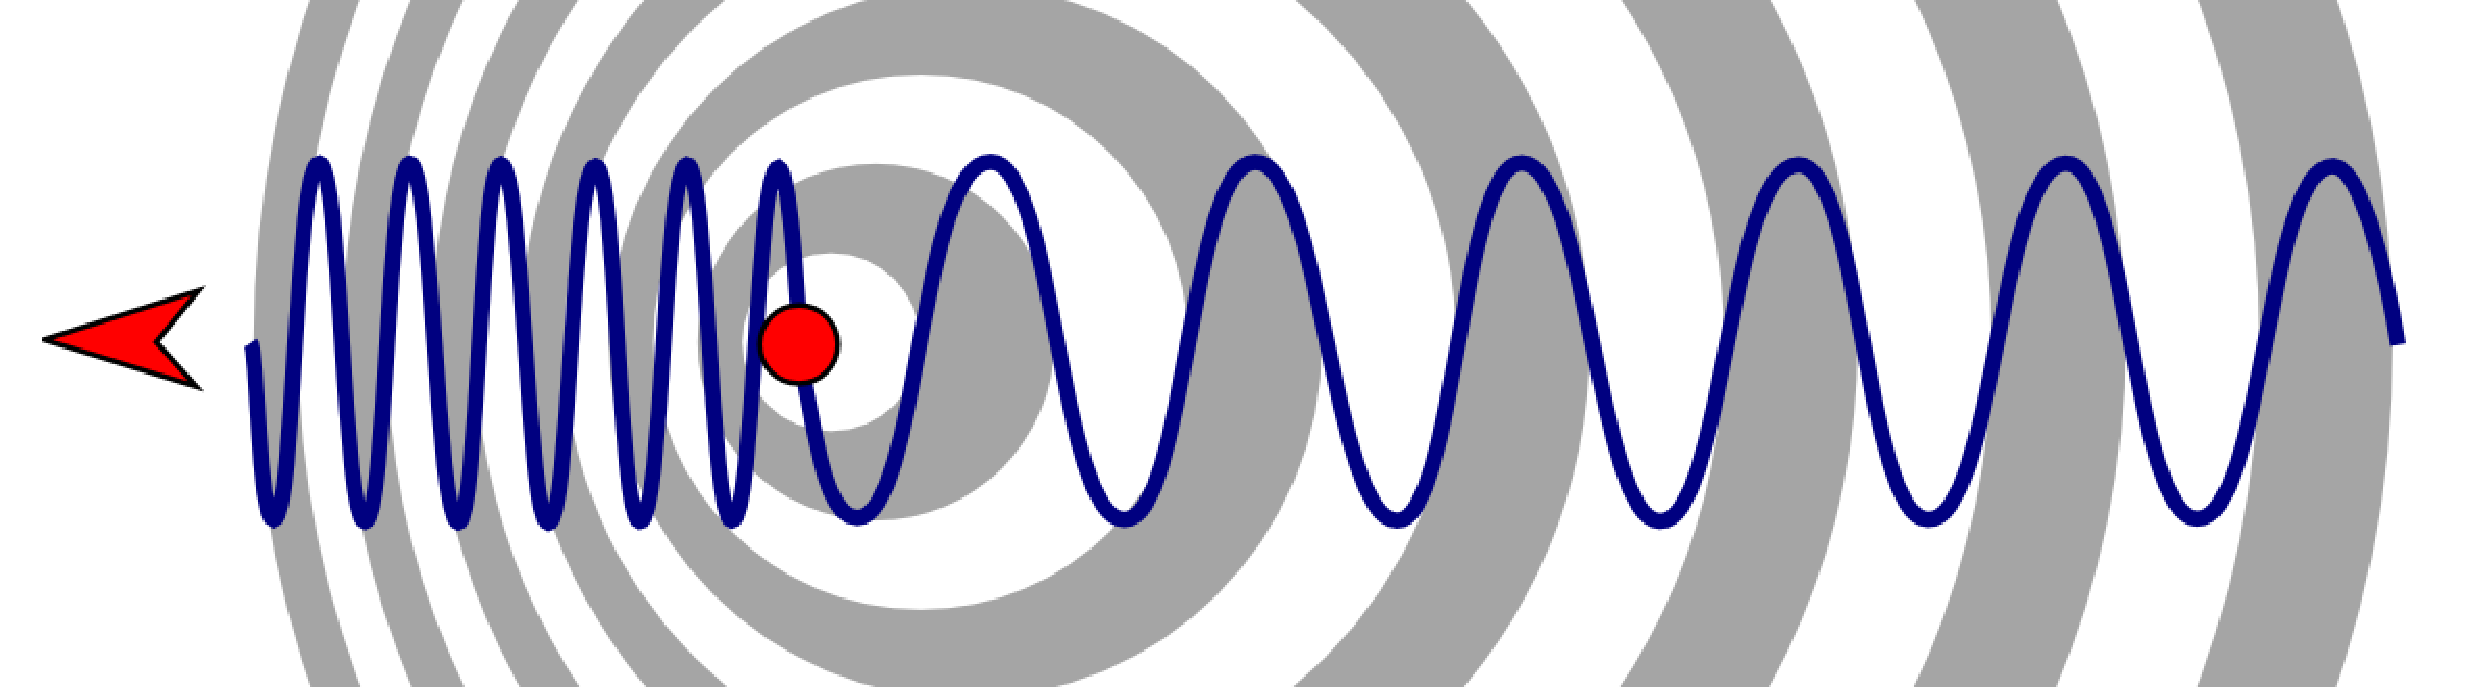
\includegraphics[width=.5\tw]{doppler-ef}
\begin{tikzpicture}
        \clip (-1.5,-0.8) rectangle + (5.5, 1.6);
        \foreach \i in {12,...,0} {
            \pgfmathsetmacro\m{int(mod(\i * 5, 2))};
            \ifthenelse{\m = 0}{
                \fill [lightgray] ($({(\i / 8)}, 0)$) circle ({0.5*5/12*\i});
            }{
                \fill [white] ($({(\i / 8)}, 0)$) circle ({0.5*5/12*\i});
            };
        };
        \filldraw (0, 0) circle (0.05);
        \draw [-latex, line width=1pt] (-1.1, 0) -- (-1.5, 0);
        \begin{axis}[
%			ylabel shift	= -1 cm,
			xmin = -1,
			xmax = 4,
			ymin=-1,
			ymax=1,
			width=6.6cm,
			height=3.6cm,
			xshift=-1cm,
			yshift=-1cm,
			grid=none,
			axis line style={draw=none},
			tick style={draw=none},
			ticks=none
			]
			
			\addplot+[domain=-1:0, samples=1000, smooth, black, line width = 1pt]{0.6*sin(deg(37.7*x))};
			\addplot+[domain=0:4, samples=200, black, line width = 1pt]{0.6*sin(deg(37.7/4*x))};
		\end{axis}
    \end{tikzpicture}

\caption{Эффект Доплера}
\label{doppler-ef}
\end{wrapfigure}
где $\lambda_0$~--- лабораторная длина волны излучения источника, а $\lambda$~--- наблюдаемая. В действительности же имеет место более общий случай: \imp{релятивистский эффект Доплера}, обусловленный проявлением СТО при $v \simeq c$, для которого формула~\eqref{eq:dopler-ef-simple} усложняется и принимает вид
\begin{equation}
\nu = \nu_0 \cdot \dfrac{\sqrt{1 - \beta^2}}{1 + \beta \cdot \cos\theta},
\label{eq:dopler-ef-rel}
\end{equation}
где $\nu$~--- частота, с которой наблюдатель принимает волны, $\nu_0$~--- частота, с которой источник испускает волны, $v$~--- скорость источника, $\theta$~--- угол между направлением на источник и вектором его скорости в системе отсчёта приёмника. Если источник радиально удаляется от наблюдателя, то $\theta = 0$, если приближается, то $\theta =\pi$. Важно, что~\eqref{eq:dopler-ef-simple} напрямую следует из \eqref{eq:dopler-ef-rel} при $\beta  \ll 1$.

\term{Красное смещение}~--- явление сдвига спектральных линий химических элементов в красную (длинноволновую) сторону, обусловленное относительным движение объектов. Параметр красного смещения определяется из наблюдаемой и лабораторной длин волн как
\begin{equation}
z = \dfrac{\lambda - \lambda_0}{\lambda_0}.
\end{equation}

Доплеровское смещение длины волны в спектре источника, движущегося с лучевой скоростью $v_{r}$ и полной скоростью $v$,
\begin{equation}
z = \dfrac{1 + v_r / c}{\sqrt{1 - \beta^2}}.
\end{equation}

\term{Гравитационное красное смещение}~--- проявление эффекта изменения частоты излучения, испущенного массивным объектом, таким как звезда или чёрная дыра. Наблюдается как сдвиг спектральных линий в спектре источника в красную область спектра. Гравитационное красное смещение определяется из формулы, выведенной Эйнштейном,
\begin{equation}
z_G=\dfrac{GM}{c^2 R}-\dfrac{GM}{c^2 r},
\label{eq:grav-red-shift}
\end{equation}
где $M$~--- масса гравитирующего тела, $R$~--- радиальное расстояние от центра масс тела до точки излучения (радиус источника), $r$~---  радиальное расстояние от центра масс источника до точки наблюдения. В случае, когда наблюдатель находится от источника много дальше его радиуса, т.\,е. выполняется соотношение $r \gg R$, выражение~\eqref{eq:grav-red-shift} можно упростить до
\begin{equation}
z_G \simeq \dfrac{GM}{c^2 R}.
\end{equation}
